\begin{frame}
\frametitle{Variedades Topológicas}
\begin{definition}[Variedad Topológica]
  Sea $M$ un espacio topológico, diremos que $M$ es una \textbf{variedad topológica de dimensión $n$} si:
  \begin{itemize}
    \item $M$ es un \textit{espacio de Hausdorff}.
    \item $M$ es \textit{segundo numerable}.
    \item $M$ es \textit{localmente euclidiano de dimensión $n$}, esto quiere decir que para cada punto $x \in M$ existe una vecindad abierta $U$ que contiene a $x$ y un homeomorfismo $\phi: U \to \phi(U)\subseteq \R^n$.
  \end{itemize}
\end{definition}\pause
\end{frame}

\begin{frame}
\centering
\begin{figure}
  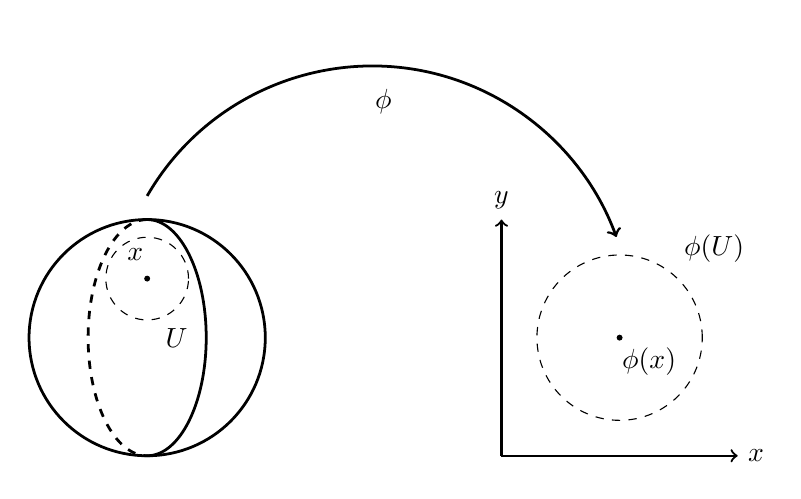
\begin{tikzpicture}[scale=1.5]
  \draw[line width=1] (-3,2) arc (90:-90:0.5 and 1);
  \draw[line width=1, dashed] (-3,2) arc (90:270:0.5 and 1);
  \draw[line width=1](-3,1) circle (1);
  \draw[color=black,thick,->] (0,0) -- (2,0) node[anchor=west]{$x$};
  \draw[color=black,thick,->] (0,0) -- (0,2) node[anchor=south]{$y$};

  \filldraw[black] (1,1) circle (0.02);
  \draw[dashed] (1,1) circle (0.7);
  \draw node at (1.25,0.80) {$\phi(x)$};
  \draw node at (1.8,1.75) {$\phi(U)$};

  \filldraw[black] (-3,1.5) circle (0.02);
  \draw node at (-3.1,1.70) {$x$};
  \draw[dashed] (-3,1.5) circle (0.35);
  \draw node at (-2.75,1) {$U$};

  \draw[line width=1, ->] (-3,2.2) arc (150:20:2.2);
  \draw node at (-1,3) {$\phi$};
\end{tikzpicture}

  \caption{Ejemplo de un homeomorfismo de una variedad a $\R^{2}$.}
\end{figure}
\end{frame}

\begin{frame}
\frametitle{Ejemplo de Variedades Topológicas}
\begin{columns}[t]
\column{.5\textwidth}
\centering
  \begin{figure}
    \scalebox{.5}{\tdplotsetmaincoords{70}{135}
\begin{tikzpicture}[scale=3,line join=bevel,tdplot_main_coords]
{\draw[color=black,thick,->] (0,0,0) -- (1,0,0) node[anchor=north east]{$x$};}%
{\draw[color=black,thick,->] (0,0,0) -- (0,1,0) node[anchor=north west]{$y$};}%
{\draw[color=black,thick,->] (0,0,0) -- (0,0,1) node[anchor=south]{$z$};}%
\end{tikzpicture}
}\\
    \caption{Los Espacios Euclidianos, $\R^n$.}
  \end{figure}
  \begin{figure}
    \scalebox{.5}{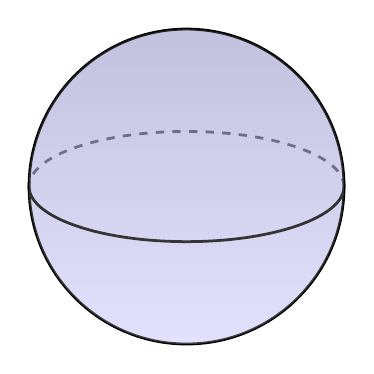
\begin{tikzpicture}[scale=2]
  \draw[line width=1, dashed] (1,0) arc (0:180:1 and 0.35);
  \draw[fill=blue!30!white!,opacity=0.5] (0,0) circle (1);
  \draw[line width=1] (1,0) arc (0:180:1 and -0.35);
  \draw[line width=1](0,0) circle (1);
  \shade[opacity=0.25] (0,0) circle (1);
\end{tikzpicture}

}\\
  \caption{Las $n-$esferas $\S^n$.}
  \end{figure}
\column{.5\textwidth}
\centering
  \begin{figure}
    \scalebox{.5}{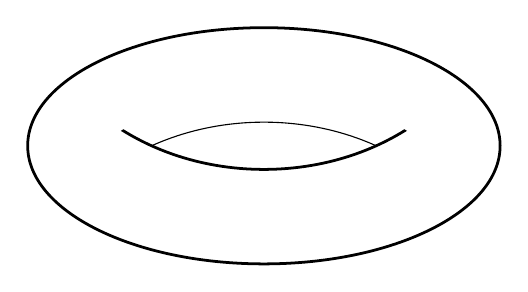
\begin{tikzpicture}
  \useasboundingbox (-3,-1.5) rectangle (3,1.5);
  \draw[line width=1] (0,0) ellipse (3 and 1.5);
  \begin{scope}
    \clip (0,-1.8) ellipse (3 and 2.5);
    \draw[line width=1] (0,2.2) ellipse (3 and 2.5);
  \end{scope}
  \begin{scope}
    \clip (0,2.2) ellipse (3 and 2.5);
    \draw (0,-2.2) ellipse (3 and 2.5);
  \end{scope}
\end{tikzpicture}
}\\
    \caption{El $n-$Toro $\mathbb{T}^n$.}
  \end{figure}
  \begin{figure}
    \centering
    \scalebox{.5}{\begin{tikzpicture}[scale=4.5]
{\draw[color=black,thick,->] (0,0) -- (1,0) node[anchor=west]{$x$};}%
{\draw[color=black,thick,->] (0,0) -- (0,1) node[anchor=south]{$y$};}%
\draw[dashed] (0.5,0.5) circle (0.25);
\filldraw[black] (0.5,0.5) circle (0.02);
\end{tikzpicture}
}\\
    \caption{Los subconjuntos abiertos\\ de las variedades.}
  \end{figure}
\end{columns}
\end{frame}

\begin{frame}
\frametitle{Ejemplo: El Espacio Proyectivo}
\centering
\begin{figure}
  \scalebox{0.75}{\begin{tikzpicture}[scale=1.75]
\draw[color=black] (-2,0) -- (2,0);
\draw[color=black] (0,-2) -- (0,2);
\draw[thick] (0,0) circle (1);
\draw[thick] (-1.5, -1.5) -- (1.5,1.5); 
\filldraw[red] (0.71,0.71) circle (0.04);
\filldraw[blue] (-0.71,-0.71) circle (0.04);
\end{tikzpicture}
}
  \caption{Representación del Espacio Proyectivo $\mathbb{RP}^{2}$}
\end{figure}
\end{frame}

\begin{frame}
\frametitle{Cartas}
\begin{definition}[Carta]
  Una \textbf{carta} en $M$ es un par ordenado $(U,\phi)$ donde $U$ es un subconjunto abierto de $M$ y $\phi$ es un homeomorfismo de $U$ a $\R^n$
\end{definition}\pause

\begin{definition}[Cartas Suavemente Compatibles]
  Si $(U,\phi)$ y $(V,\psi)$ son dos cartas en $M$ tales que $U \cap V \neq \varnothing$, llamaremos \textbf{mapa de transición} a la composición:
  \[ \psi \circ \phi^{-1}: \phi(U \cap V) \to \psi(U \cap V) \]
  
  y además diremos que las cartas $(U,\phi)$ y $(V,\psi)$ son \textbf{suavemente compatibles} si $U \cap V = \varnothing$ o si el mapa de transición $\psi \circ \phi^{-1}$ es un difeomorfismo.
\end{definition}
\end{frame}

\begin{frame}
\end{frame}

